\section{Results}\label{sec:short_results}

\subsection{Where the integration correction grows}
Figure~\ref{fig:short_mechanism} maps the synthetic evidence. Corrections are largest where historical information is weak and the pricing function has substantial volatility curvature. High volatility, long horizons, extreme moneyness, and limited realized fixing produce the strongest effects in the evaluated states. The largest absolute correction is \$0.1384 per barrel on the normalized \$100 forward; the largest cell-level 99th percentile is \$0.1271. These are observed simulation magnitudes, not bounds on all possible contract states.

The second-order approximation closely tracks the cell-level mean correction, with correlation 0.9995 and through-origin slopes close to one in the most adverse cells. This agreement links the measured correction to posterior variance and volatility curvature rather than to an unexplained difference between estimators.

Partial fixing generally reduces the correction as less of the average remains stochastic, but the relationship is not uniformly monotone. In Figure~\ref{fig:short_mechanism}C, the 252-day case initially increases before declining. Fixing additional observations changes both volatility exposure and the curvature of the residual option value. The integration effect therefore depends on the remaining payoff state, as well as on uncertainty in the volatility estimate.

\begin{figure*}[!tb]
\centering
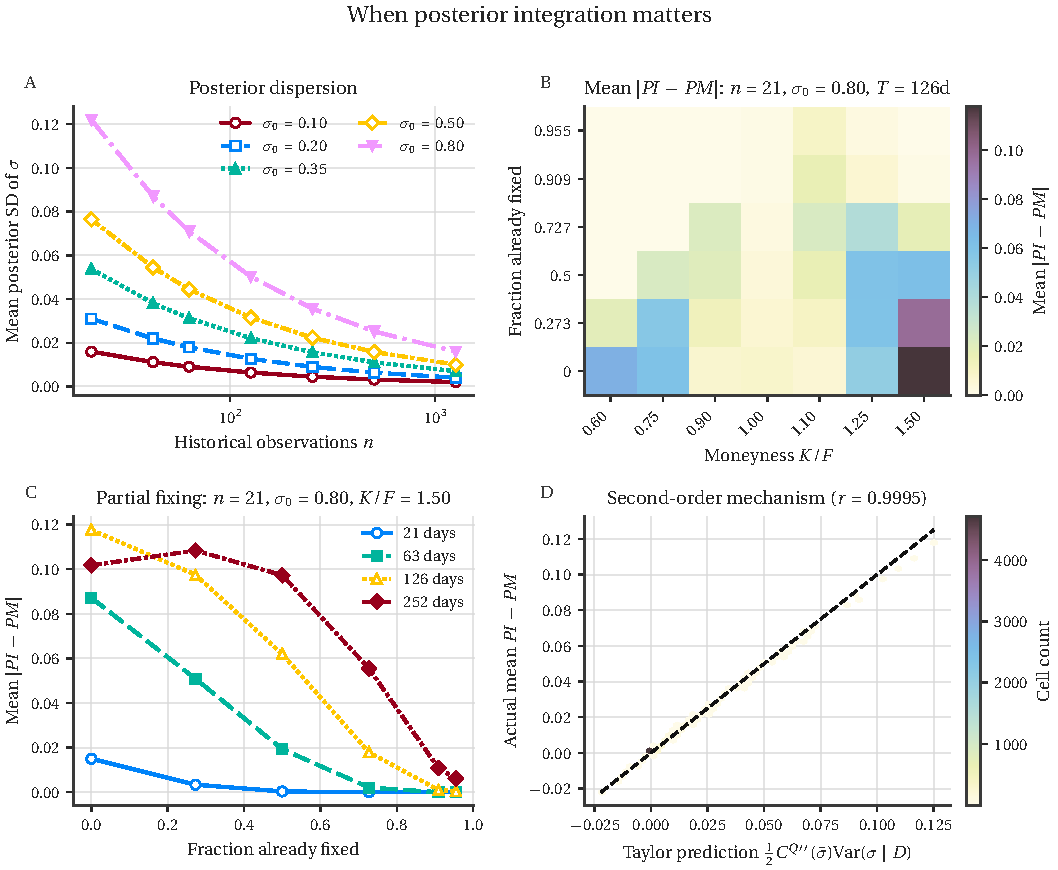
\includegraphics[width=\textwidth]{figures/publication/fig01_mechanism_map.pdf}
\caption{Posterior integration across synthetic WTI-like states. Panel A shows posterior dispersion against historical sample size. Panels B and C show absolute PI--PM corrections by moneyness and partial fixing. Panel D compares cell-level mean corrections with Equation~\eqref{eq:short_taylor}; the correlation is 0.9995. Cell count records the number of scenario cells in each hexagonal bin.}\label{fig:short_mechanism}
\end{figure*}

\subsection{A small point correction with wider posterior price intervals}
Table~\ref{tab:short_october} reports the October-2026 baseline. PI and PM have nearly identical settlement-pricing errors. More directly, their mean absolute difference is \$0.000745 per barrel, while the mean central 95\% posterior model-price interval width is \$0.2733 per barrel. The interval width is about 367 times the correction, illustrating their different scales rather than defining a universal uncertainty ratio.

\begin{table}[!t]
\centering
\caption{October-2026 pricing and posterior model-price uncertainty, on 310 contract-date observations over 12 dates. Values are U.S. dollars per barrel. PI and PM use the same Monte Carlo pricing model; interval widths come from the historical-volatility posterior.}\label{tab:short_october}
\begin{tabular}{lr}
\toprule
Quantity & Value\\
\midrule
PI RMSE & 0.5177\\
PM plug-in RMSE & 0.5183\\
Mean absolute PI--PM correction & 0.000745\\
Mean 95\% posterior interval width & 0.2733\\
\bottomrule
\end{tabular}
\end{table}

The small correction follows the local mechanism: averaging a relatively concentrated posterior through this pricing function shifts its mean little. The wider price intervals reflect uncertainty that remains around the conditional value. Both historical-volatility point prices understate settlements on average in the October panel. Integrating the same posterior does little to remove that shared pricing discrepancy.

\begin{figure*}[!tb]
\centering
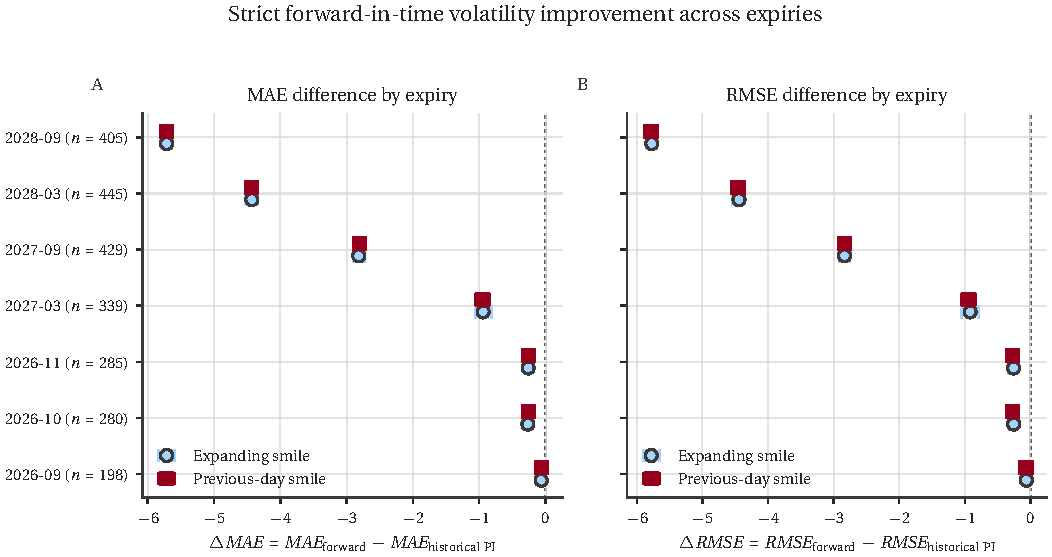
\includegraphics[width=\textwidth]{figures/publication/fig03_forward_q_cluster_bootstrap.pdf}
\caption{Pricing-error differences by APO expiry. Negative values indicate lower error for earlier-date APO implied volatility than for historical PI. Bars show 95\% percentile intervals from valuation-date cluster resampling. Volatility estimates use only earlier option dates; repricing conditions on the current futures curve and realized fixings.}\label{fig:short_forward_bootstrap}
\end{figure*}

\begin{table*}[!tb]
\centering
\caption{Earlier-date volatility information and later-date APO valuation. Panel A uses 2,381 exact common holdouts over 15 dates. Panel B uses the 2,366 observations with earlier IV for the same contract. MAE and RMSE are U.S. dollars per barrel. Historical PI is the canonical Monte Carlo baseline; scalar historical, GARCH, and option-implied inputs use Curran repricing.}\label{tab:short_forward}
\begin{tabular}{lrr}
\toprule
\multicolumn{3}{c}{Panel A: volatility inputs on the main holdouts}\\
Volatility input & MAE & RMSE\\
\midrule
Historical PI & 2.6187 & 3.4090\\
Rolling 63 returns & 4.5201 & 5.6465\\
Horizon-matched GARCH(1,1) & 2.6730 & 3.4441\\
Previous-day APO smile & 0.1075 & 0.1594\\
\midrule
\multicolumn{3}{c}{Panel B: same-contract persistence on exact common rows}\\
Volatility input & MAE & RMSE\\
\midrule
Historical PI & 2.6279 & 3.4173\\
Same-contract lagged IV & 0.0992 & 0.1403\\
Previous-day fitted APO smile & 0.1074 & 0.1594\\
\bottomrule
\end{tabular}
\end{table*}

\subsection{Volatility information dominates the evaluated historical comparators}
Table~\ref{tab:short_forward} compares volatility inputs on exact common samples. On the 2,381 holdouts, the historical PI baseline has RMSE 3.4090. The evaluated rolling estimators and EWMA do not improve on it; the strongest rolling comparator uses 63 returns. Horizon-matched GARCH has RMSE 3.4441, close to the expanding historical baseline. The full historical comparison appears in Section S1.

Prior APO option information produces substantially smaller errors. The previous-day smile has RMSE 0.1594, and the expanding earlier-date smile has RMSE 0.1725. Figure~\ref{fig:short_forward_bootstrap} shows improvements across all seven admitted expiries, with valuation-date bootstrap intervals below zero for the reported error differences.





Panel B explains part of that result. Carrying forward the same contract's earlier IV yields lower pooled error than fitting the previous-day smile. This descriptive ranking shows that the historical-versus-option-implied improvement does not require flexible cross-sectional smoothing. Persistence of option-implied states, combined with current-state repricing, is sufficient to reproduce it on these rows. The comparison does not establish general superiority of IV carry over fitted smiles.



\subsection{The option-implied improvement transfers across instruments}
Table~\ref{tab:short_lo} moves the volatility source outside the APO family. On 253 exact common-support observations, prior vanilla-WTI IV reduces RMSE from 0.5562 for historical PI to 0.2599. The corresponding prior APO smile has RMSE 0.2686. Date-cluster bootstrap intervals support the external improvement over historical volatility, while LO-versus-APO differences are smaller and are not uniformly distinguishable across MAE and RMSE.

\begin{table}[!t]
\centering
\caption{External volatility information on 253 October-2026 APO observations over 10 dates within prior LO moneyness support. Errors are U.S. dollars per barrel. Historical PI uses Monte Carlo; option-implied values use Curran. LO and APO volatility inputs use strictly earlier option dates.}\label{tab:short_lo}
\begin{tabular}{lrr}
\toprule
Volatility input & MAE & RMSE\\
\midrule
Historical PI & 0.4464 & 0.5562\\
Previous-day vanilla-WTI IV & 0.1559 & 0.2599\\
Previous-day APO IV & 0.1676 & 0.2686\\
\bottomrule
\end{tabular}
\end{table}

The external experiment follows the established commodity calibration logic of \citet{shirayatakahashi2011}, using earlier vanilla information in the present scalar model. Its role is to show that the improvement is not confined to reusing earlier prices from the target option family. Together with the persistence comparator, it identifies option-implied volatility as the larger empirical point-pricing margin in the evaluated samples.
